\documentclass[11pt]{article}
\usepackage{inputenc}
\usepackage{comment}
\usepackage{fontspec}
\usepackage{authblk}
\usepackage{graphicx}
\usepackage{fancyhdr}
\usepackage{amssymb}
\usepackage{amsmath}
\usepackage{gensymb}
\usepackage{float}
\usepackage{enumerate}
\usepackage{tocloft}
\usepackage{abstract}
\usepackage[hidelinks]{hyperref}
\usepackage{appendix}
\usepackage[dvipsnames, svgnames, x11names]{xcolor}
\usepackage{dirtree}
\usepackage{cite}
\usepackage{geometry}
\usepackage{makecell}
\usepackage{multirow}
\usepackage{graphicx}
\usepackage{float}
\usepackage{subfig}
\usepackage[ruled]{algorithm2e}
\usepackage{indentfirst}
\usepackage{unicode-math}
\usepackage{afterpage}
\usepackage{tikz}

% \setlength{\headheight}{16pt}

\usepackage{setspace}
\doublespacing

\setmainfont{Times New Roman}

% \setmainfont[%
% ItalicFont=NewCM10-Italic.otf,%
% BoldFont=NewCM10-Bold.otf,%
% BoldItalicFont=NewCM10-BoldItalic.otf,%
% SmallCapsFeatures={Numbers=OldStyle}]{NewCM10-Regular.otf}

% \setsansfont[%
% ItalicFont=NewCMSans10-Oblique.otf,%
% BoldFont=NewCMSans10-Bold.otf,%
% BoldItalicFont=NewCMSans10-BoldOblique.otf,%
% SmallCapsFeatures={Numbers=OldStyle}]{NewCMSans10-Regular.otf}

% \setmonofont[ItalicFont=NewCMMono10-Italic.otf,%
% BoldFont=NewCMMono10-Bold.otf,%
% BoldItalicFont=NewCMMono10-BoldOblique.otf,%
% SmallCapsFeatures={Numbers=OldStyle}]{NewCMMono10-Regular.otf}

% \setmathfont{NewCMMath-Regular.otf}

\pagestyle{fancy}

\renewcommand\thesection{\arabic{section}}

\newcommand*{\rmd}{\mathop{}\!\mathrm{d}}
\newcommand*{\sgn}{\mathrm{sgn}}
\renewcommand{\cftsecleader}{\cftdotfill{\cftdotsep}}

\title{\vspace{-1.5cm} \huge Stock Volatility Forecasting and Word Features Selection --- Based On 10-K Corpus}

\author{
  \parbox{0.3\textwidth}{
    \centering WANG Zeyu
    \vspace{.25cm}
  }
  \parbox{0.3\textwidth}{
    \centering LIU Chang
    \vspace{.25cm}
  }
  \parbox{0.3\textwidth}{
    \centering TAN Huangao
    \vspace{.25cm}
  }
  \parbox{0.3\textwidth}{
    \centering LI Borui
  }
  \parbox{0.3\textwidth}{
    \centering ZHU Xinqi
  }
  \parbox{0.3\textwidth}{
    \centering GAO Yifeng
  }
}

\date{\today}

\setcounter{tocdepth}{2}
\setcounter{secnumdepth}{3}

\begin{document}

\maketitle
\thispagestyle{empty}
\setcounter{page}{0}

\begin{abstract}
  As a key indicator of the market risk, the stock volatility is an important evidence to support the investment portfolio. The traditional time series models such as GARCH models only rely on the volatility, but ignore the unstructured text data like companies' 10-K reports, which is also shown to be helpful in forecasting. However, due to the complexity of natural language and the evolving semantic patterns, it is still challenging to extract operable signals from the narration of natural language. Focusing on exploring the relation between the 10-K report and stock volatility, we apply Lasso regression, Ridge regression, and the decision tree on the companies' 10-K reports together with historical volatility, to predict the future volatility. The result shows that it can perform much better than the Naive model. Meanwhile, based on the word features given by the models, we also explore the difference of word features between the years and models and found it changes due to some big events.
  \\\\
  \textbf{Keywords:} keywords
\end{abstract}

\newpage

\section{Introduction}

The effective transmission and interpretation of qualitative information in financial markets play a key role in shaping investor behavior and dynamic asset pricing. As a key indicator to measure market risk, stock volatility includes uncertainty and different expectations of investor for stock investment \cite{RePEc:eee:finlet:v:69:y:2024:i:pb:s1544612324011929} . As the traditional quantitative models mainly rely on structured financial data (such as historical prices and accounting ratios), unstructured text data has shown an explosive growth trend in the Internet era, especially in the aspect of company disclosure, which provides untapped potential for enhancing volatility prediction \cite{Ma2024} . Although it has information value, due to the complexity of natural language and the evolving semantic patterns in the annual report, it is still challenging to extract operable signals from the narration of natural language. Previous studies have established a preliminary link between text sentiment and short-term market response \cite{li2022sentiment} , but the dynamic interaction between lexical features and long-term fluctuations, as well as the temporal stability of these features, have not been fully explored. This gap not only limits the improvement of prediction model, but also hinders the optimization of corporate disclosure practice and regulatory supervision.

\subsection{Motivation and Goal}

The motivation for this study is driven by four interconnected objectives that bridge practical financial applications, corporate governance, and academic innovation. First, we seek to decode market information transmission mechanisms by analyzing the impact of unstructured textual data in 10-K reports --- particularly the Management's Discussion and Analysis (MD\&A) section \cite{brown2024financial}  --- on stock volatility. This investigation validates whether financial markets rapidly and accurately internalize qualitative disclosures, thereby shedding light on how investors interpret textual information to inform trading decisions. Second, our work aims to construct quantitative investment strategies by identifying key lexical features within 10-K filings. By developing data-driven models to predict short-term stock volatility and flagging risk-indicative terms (e.g., negative sentiment words), we provide tools for portfolio optimization and preemptive risk mitigation \cite{ta2020portfolio} . Third, this research addresses corporate governance and disclosure quality enhancement \cite{RAJENDRAN2024101813} . By pinpointing textual patterns that disproportionately influence market reactions --- such as ambiguous or exaggerated language --- we offer actionable insights for firms to refine their communication strategies. Concurrently, regulators can leverage these findings to detect deliberate obfuscation of risks in corporate disclosures, fostering greater transparency. Finally, this study contributes to academic research by pioneering methodologies at the intersection of finance and computational linguistics. By advancing text-based volatility forecasting frameworks, we enrich interdisciplinary dialogue and establish novel paradigms for analyzing financial narratives. Collectively, these objectives underscore the transformative potential of integrating textual analytics into financial decision-making, risk management, and regulatory oversight.

Based on the motivation of the above experiment, this study mainly pursues the following research objectives. First of all, we hope to predict the logarithmic volatility of stock returns in the next year by studying the MD\&A part of the form 10-K report \cite{MATTERA20241539}\cite{ma2023stock} . We will use the machine learning model including Lasso/Ridge regression and decision tree, and combine NLP technology \cite{yogatama2015sparse} to extract semantic features from unstructured text. The second goal is to identify and evaluate the importance of a single token in predicting volatility, focusing on its time stability. Through pseudo-inverse decomposition of NMF components \cite{fu2019nonnegative} and feature selection metrics, we separated the first 1000 words that were most closely related to volatility changes. This allows us to check whether the forecast terms (e.g., risk related phrases) are consistent in different years or change with regulatory changes.

These objectives aim to establish an effective framework for text driven volatility reduction, reveal operable language patterns, and provide effective information for investment strategies, company disclosures and regulatory practices.

\subsection{Datasets}

To achieve these objectives, we leverage a curated subset of the 10-K Corpus \cite{Kogan2009} , spanning annual filings from 1996 to 2005.In the original data set, the data of these two parts have better value for research. First, the tokenized MD\&A sections(e.g., 1996.tok.tgz), which is the most directly related component used for prediction in Form 10-K.It provides the insights of management on the financial condition of company, changes in financial condition and overall operation. This section contains forward-looking statements, risk disclosures and strategic insights, which are not available in other parts of the report. Therefore, this section provides a rich source of information for predicting future stock volatility. Feature extraction can help us understand the transmission mechanism of market information. The second part is corresponding annualized log volatility metrics derived from stock returns, aligned temporally with the 10-K reporting cycle(e.g., 1996.logvol.-12.txt).

\section{Methods}

\subsection{Text preprocessing}

We use the Natural Language Toolkit (NLTK) \cite{nltk-py} as lemmatizer, stemmer and stop token filter with the idea that: (1) Some words are regarded as insignificant in text analysis, e.g. a, an, the, above, across; (2) Words appear in several inflected forms but with same meaning should be considered as the same, e.g. the words achieves, achieved, achievement, achievements are the same and we transform them to the root achiev. This method can greatly reduce our data processing volume and help to reduce the memory and time usage.

\subsection{Term Frequency–Inverse Document Frequency (TF-IDF)}

The term frequency–inverse focument frequency (TF-IDF) \cite{sparck1972statistical}\cite{robertson2004understanding} measures the importance of a word to a document in corpus via

$$
  \begin{aligned}
     & \text{(Term frequency)}             & \mathrm{tf}(t, d)  & = \frac{f_{t, d}}{\sum_{t^\prime \in d} f_{t^\prime, d}},                                     \\
     & \text{(Inverse document frequency)} & \mathrm{idf}(t, d) & = \log_2\left( \frac{N}{\left\vert \left\{ d: d \in D, t \in d \right\} \right\vert} \right),
  \end{aligned}
$$

where $f_{t, d}$ is the raw count of a term $t$ in a document $d$, and $N$ is the total number of documents. After computing the TF-IDF, each company is represented by a vector where each element corresponds to a token's TF-IDF weight, highlighting discriminative keywords.


\subsection{Nonnegative Matrix Factorization (NMF)}

In order to further reduce the dimension of the input data, we use the nonnegative matrix factorization (NMF) \cite{lee2000algorithms} , with which we can decomposes the TF-IDF matrix $X \in \mathbb{R}^{n \times m}$ into two nonnegative smaller matrices $W \in \mathbb{R}^{n \times d}$ and $H \in \mathbb{R}^{d \times m}$, where $X \approx W H$ and $d$ is the given number of dimension.

The previous research \cite{lee1999learning} have shown that this method is particularly suitable for text data due to non-negativity and is able to learn the semantic features of text, which allows us to extract interpretable latent topics that capture the underlying themes in the MD\&A sections. Besides, unlike other dimensionality reduction techniques like PCA, NMF provides sparse and parts-based representations, making it easier to identify meaningful topics and understand the contribution of individual words.

\subsection{Naive Model (Baseline)}

The previous research \cite{beck2025mind} has shown that the naive model is better than many other complex models, especially for high-volatility time series. Thus we choose the naive model (or Persistence model) as our baseline, which uses the current (or same period) value as the forecast. Since it only requires the  doesn't involve the word features or any assumptions.

\subsection{Lasso/Ridge Regression \& Decision Tree}

The models we used are Lasso regression, Ridge regression and Decision Tree. These models (also their extensions) are powerful in forecast and can have better performance compare with other models like heterogeneous autoregressive (HAR) models \cite{liang2023forecasting} \cite{li2022forecasting} \cite{christensen2023machine}. In addition, they are well-known inherently interpretable, which can help us extract whether a word implies the increasing or decreasing of volatility.

\subsection{Model Evaluation}

The two widely used measurement MAE and MSE will be used to evaluate the results where they are computed as

$$
  \begin{aligned}
    \text{MAE}(x, \hat{x}) & = \frac{1}{N} \sum_{i=1}^N \vert x_i - \hat{x}_i \vert, \\
    \text{MSE}(x, \hat{x}) & = \frac{1}{N} \sum_{i=1}^N  (x_i - \hat{x}_i)^2.        \\
  \end{aligned}
$$

Another problem we are interested in is the words features. We first compute the weight of each words via the pseudo inverse of $H$ with

$$
  H^+ \beta = (V^T \Lambda^+ U) \beta,
$$

where $\beta \in \mathbb{R}^d$ is the model parameter and $H \in \mathbb{R}^{d \times m}$ is components by NMF. Here the pseudo inverse $H^+$ is calculate from the SVD that $H = U^T \Lambda V$, and $\Lambda^+$ is the diagonal matrix consisting of the reciprocals of $H$'s singular values. In order to compare the features cross models and years, we selected the top $1000$ words (about $1\% \sim 5\%$ of total) for each model and check whether they are similar between different methods and years.

\subsection{Overview}

\begin{figure}
  \centering
  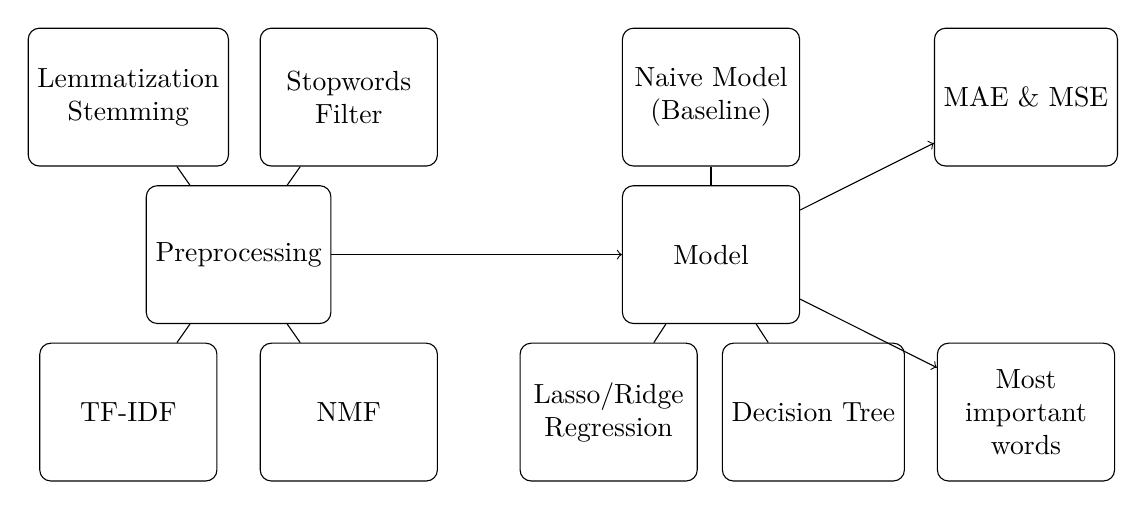
\begin{tikzpicture}[minimum width=2.25cm, minimum height=1.75cm]
    \node[draw, align=center, rounded corners]  (P)   at ( 0.0,  0.0)    {Preprocessing};
    \node[draw, align=center, rounded corners]  (LS)  at (-1.4,  2.0)    {Lemmatization \\ Stemming};
    \node[draw, align=center, rounded corners]  (SF)  at ( 1.4,  2.0)    {Stopwords \\ Filter};
    \node[draw, align=center, rounded corners]  (T)   at (-1.4, -2.0)    {TF-IDF};
    \node[draw, align=center, rounded corners]  (N)   at ( 1.4, -2.0)    {NMF};

    \node[draw, align=center, rounded corners]  (M)   at ( 6.0,  0.0)     {Model};
    \node[draw, align=center, rounded corners]  (NM)  at ( 6.0,  2.0)    {Naive Model \\ (Baseline)};
    \node[draw, align=center, rounded corners]  (LR)  at ( 4.7, -2.0)    {Lasso/Ridge \\ Regression};
    \node[draw, align=center, rounded corners]  (D)   at ( 7.3, -2.0)    {Decision Tree};

    \node[draw, align=center, rounded corners]  (E)   at (10.0,  2.0)   {MAE \& MSE};
    \node[draw, align=center, rounded corners]  (W)   at (10.0, -2.0)   {Most \\ important \\ words};

    \draw[->] (P) -- (M);

    \draw[-] (P) -- (LS);
    \draw[-] (P) -- (SF);
    \draw[-] (P) -- (T);
    \draw[-] (P) -- (N);

    \draw[-] (M) -- (NM);
    \draw[-] (M) -- (LR);
    \draw[-] (M) -- (D);

    \draw[->] (M) -- (E);
    \draw[->] (M) -- (W);
  \end{tikzpicture}
  \caption{Overview flowchart for our method.}
  \label{figure-flowchart}
\end{figure}

The Figure \ref{figure-flowchart} is an overview of our method. The number of the components by NMF is set to $20$ balancing the memory, time and the accuracy. Consider the number that coefficients close to zero and the model error, the penalty for the Lasso is $0.00005$ and $1.0$ for Ridge, meanwhile, the depth of the tree is set to $5$.

Then we test the model in two approaches. First we choose the data from one or several years, and split them into training dataset ($80\%$) and test dataset ($20\%$). In this case, the model is trained and tested on the data from same years, thus to avoid the flukes cause by splitting, we repeat the experiment for $400$ times, with the central limit theorem and sample variance, we can control the error under $0.003$ (with the probability over $95\%$), which is enough accurate.

Another test is to train the model via the data from one or several years and forecast the following year. In this case, we use all the data from previous years as the training set and the whole following year's data as the testing set. This approach will be run once to show the model's ability to deal with the new text data.

\section{Result}

\subsection{Forecasting error}

\subsubsection{Model trained by 1-year training data}

We first train the data with 1-year text data and volatility. The Figure \ref{figure-1-year-test} shows the error of the model predicting the volatility in the same year, while the Figure \ref{figure-1-year-pred} shows the error of the prediction with the text and volatility of the next year.

\afterpage{
  \clearpage
  \begin{figure}[H]
    \centering
    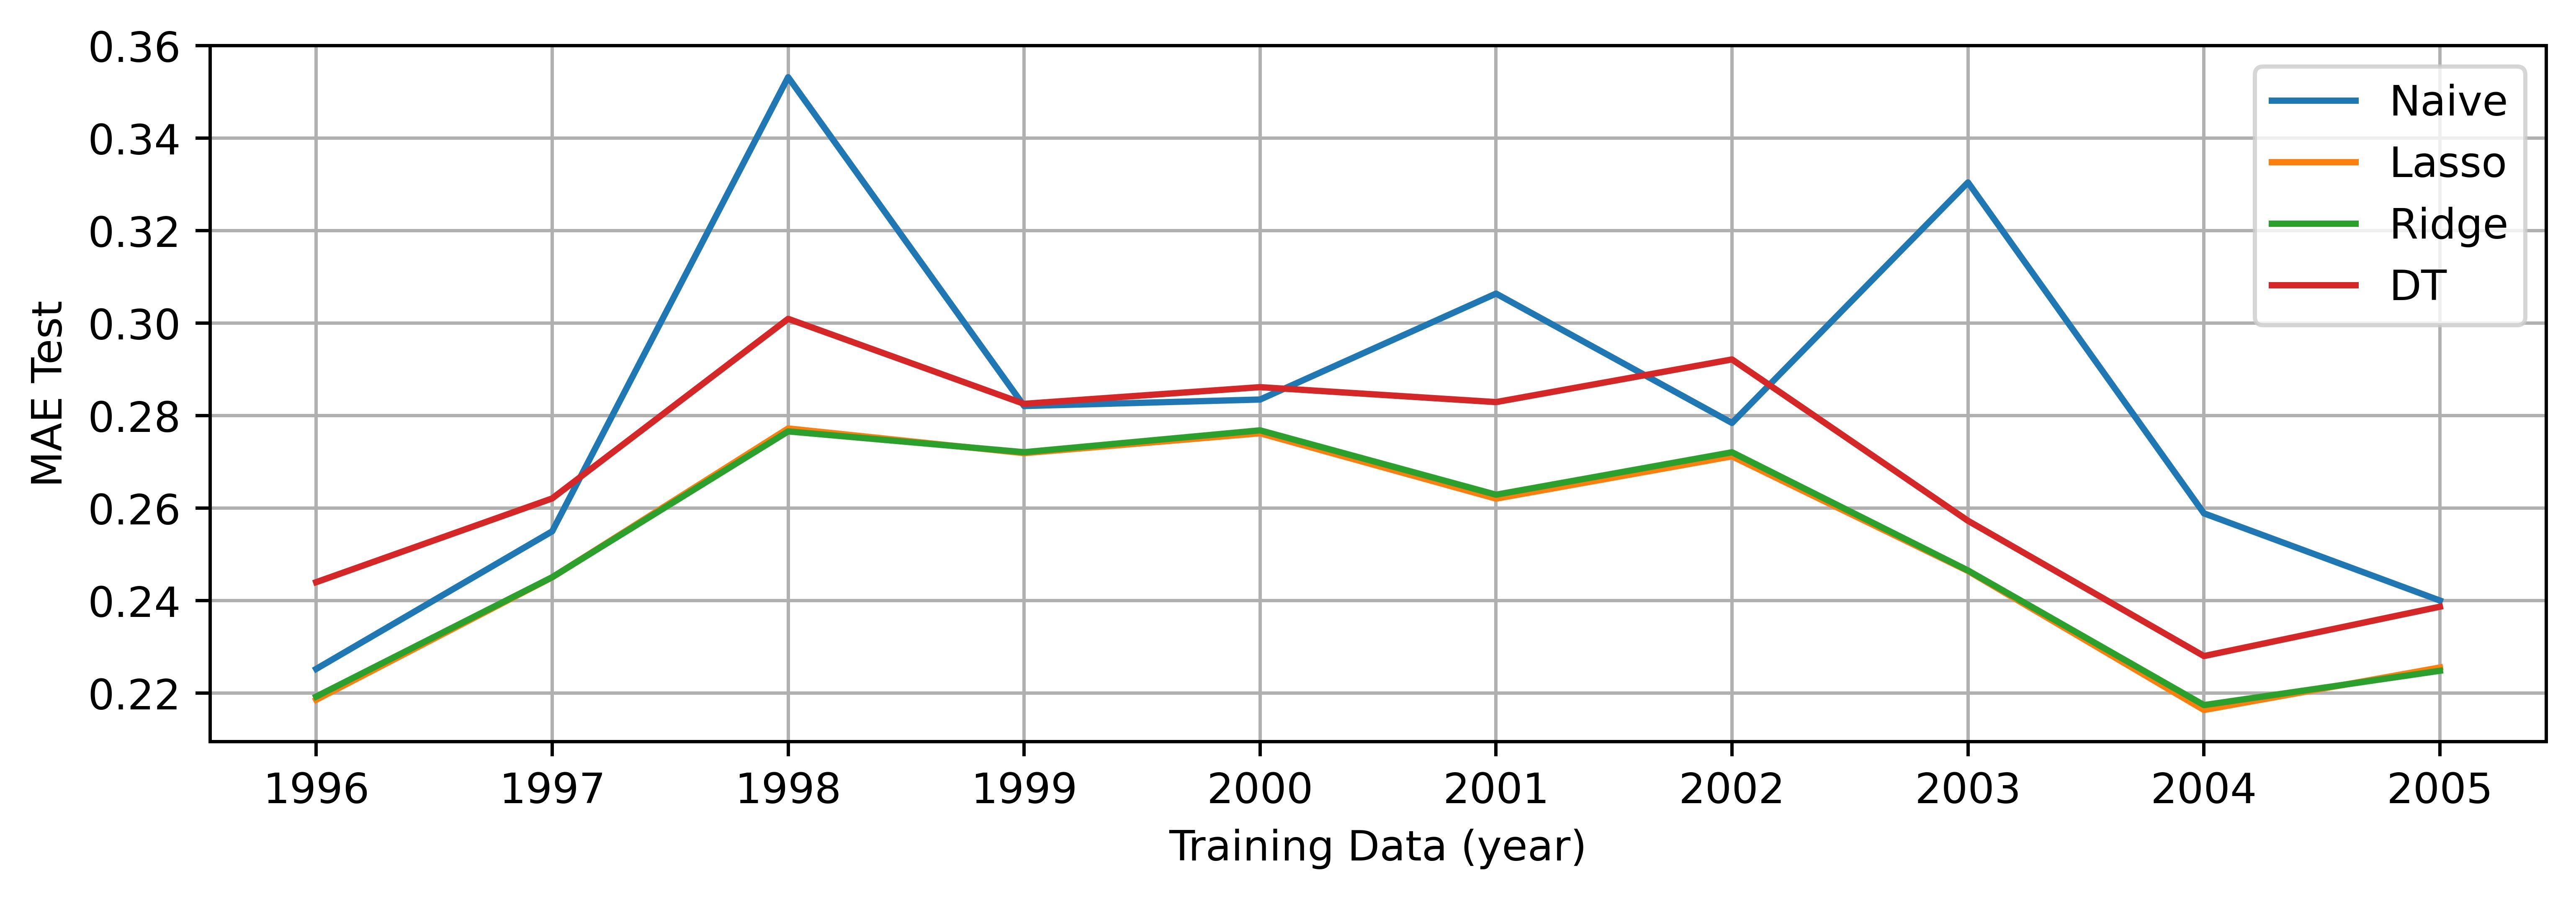
\includegraphics[width=0.7\textwidth]{../Result/Res-1_MAE_test.jpg} \\
    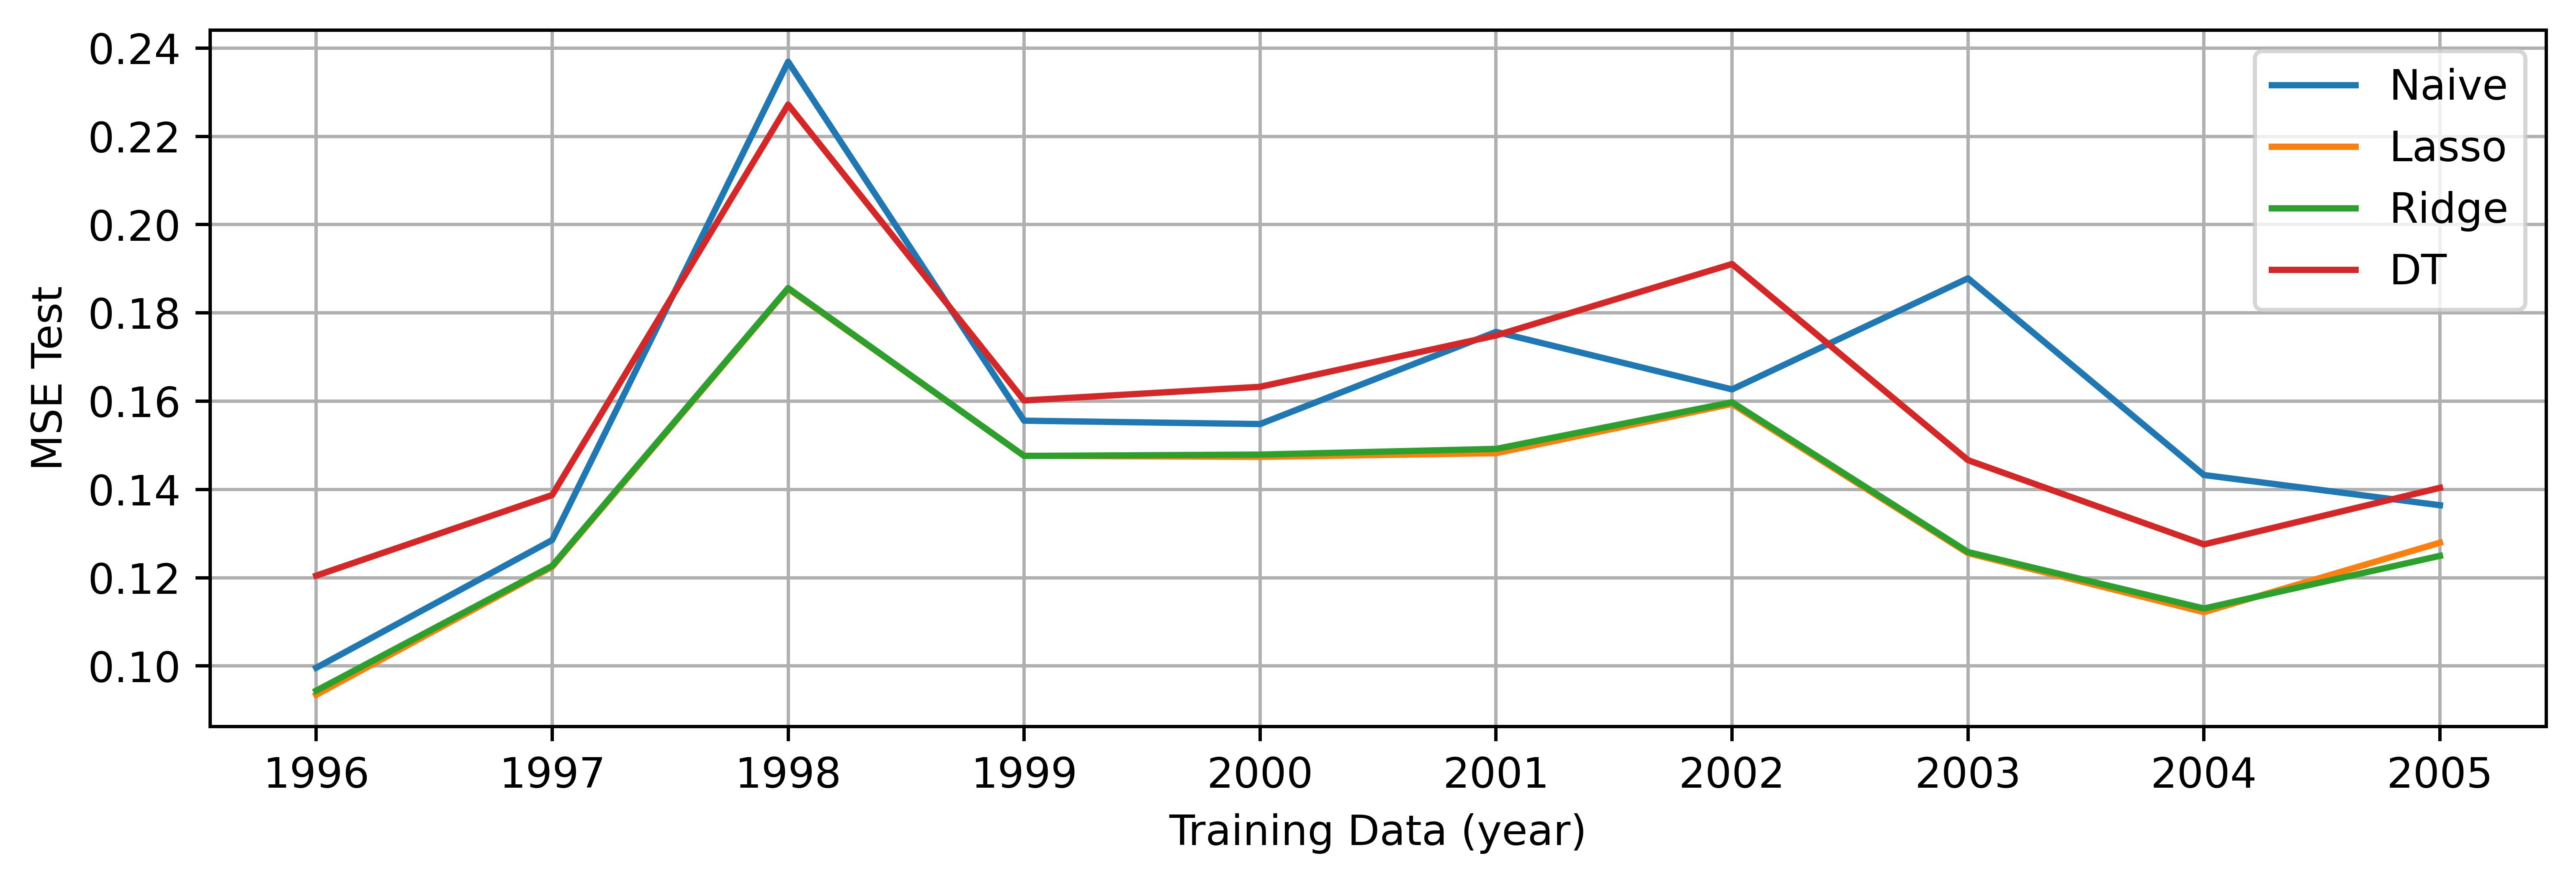
\includegraphics[width=0.7\textwidth]{../Result/Res-1_MSE_test.jpg}
    \caption{MAE and MSE for predicting the 1-year's data with the model trained by the same 1-year's data.}
    \label{figure-1-year-test}
  \end{figure}

  \begin{figure}[H]
    \centering
    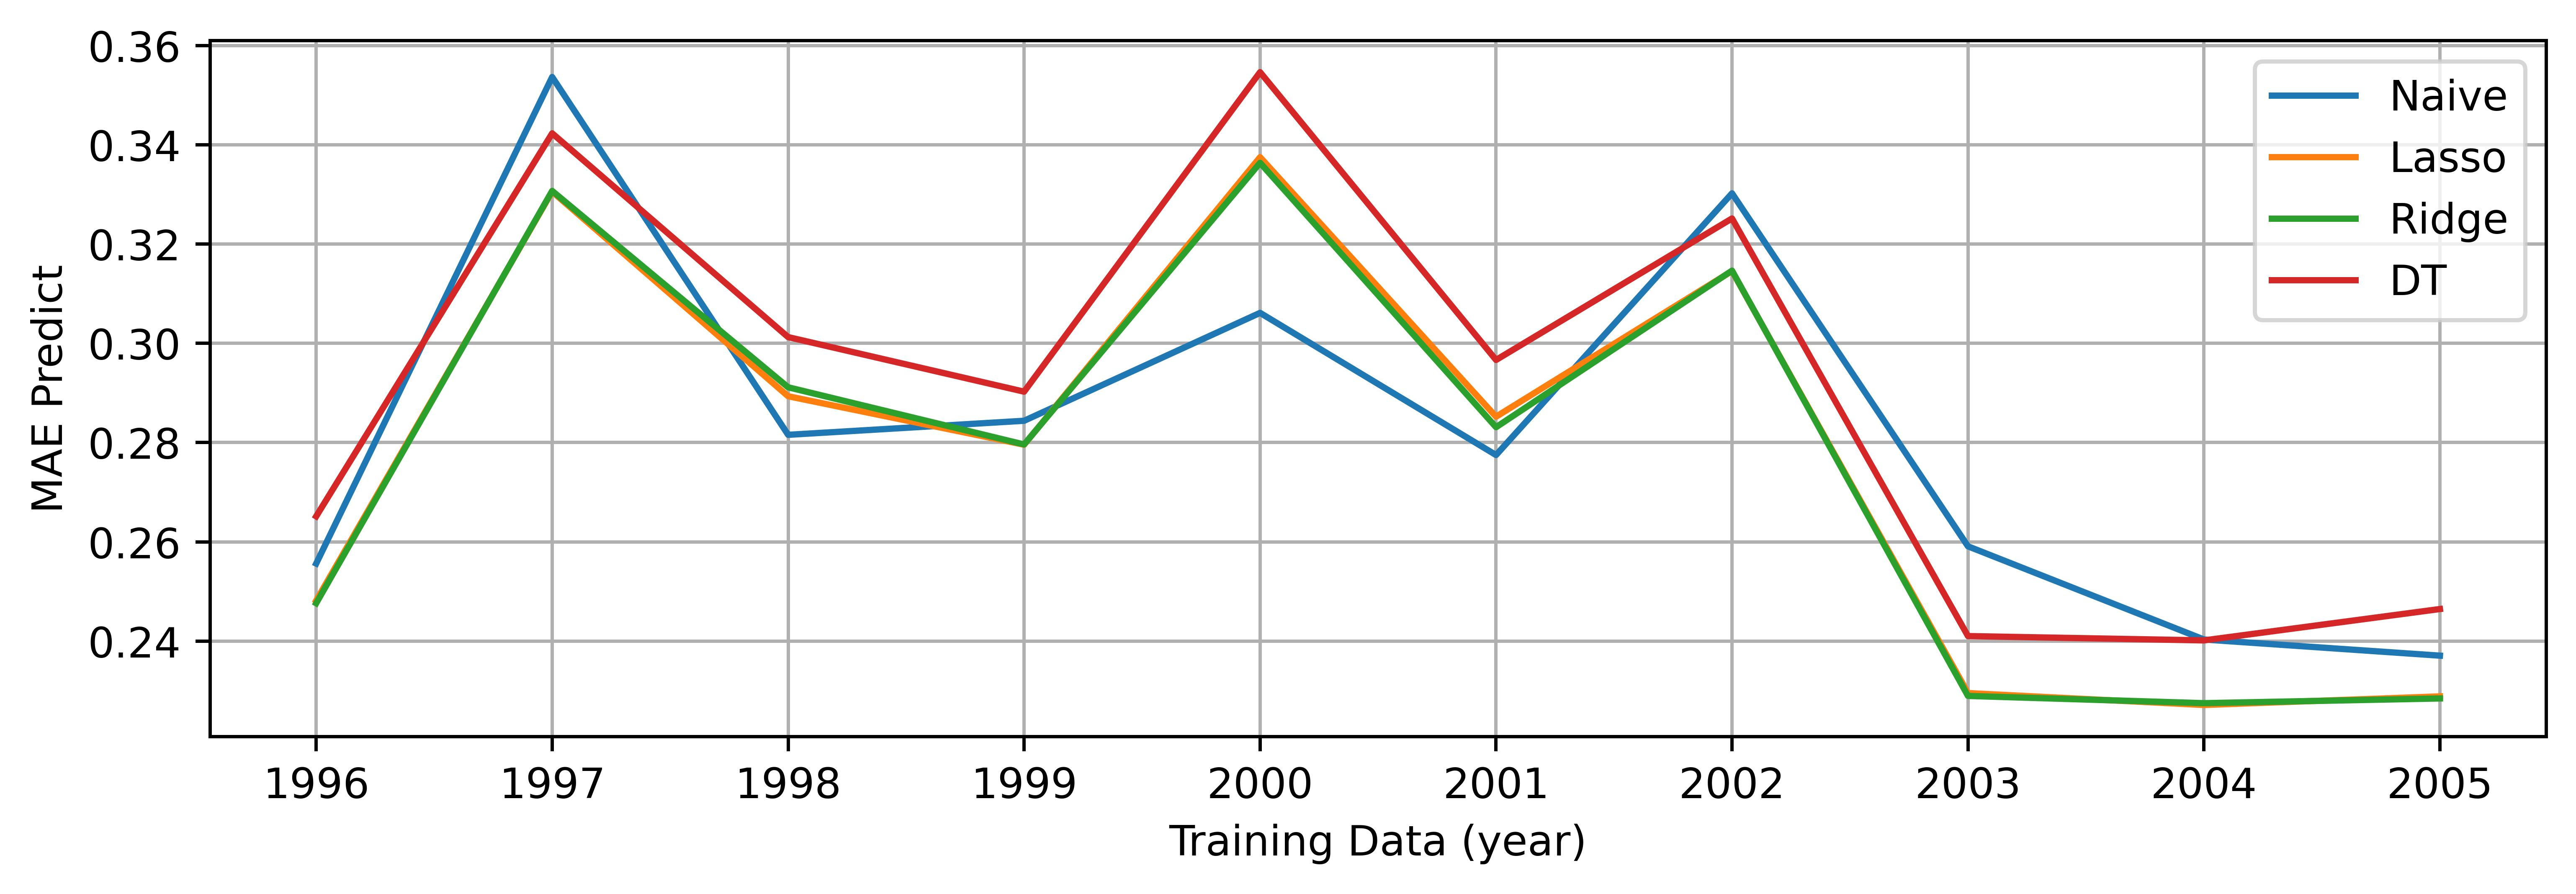
\includegraphics[width=0.7\textwidth]{../Result/Res-1_MAE_pred.jpg} \\
    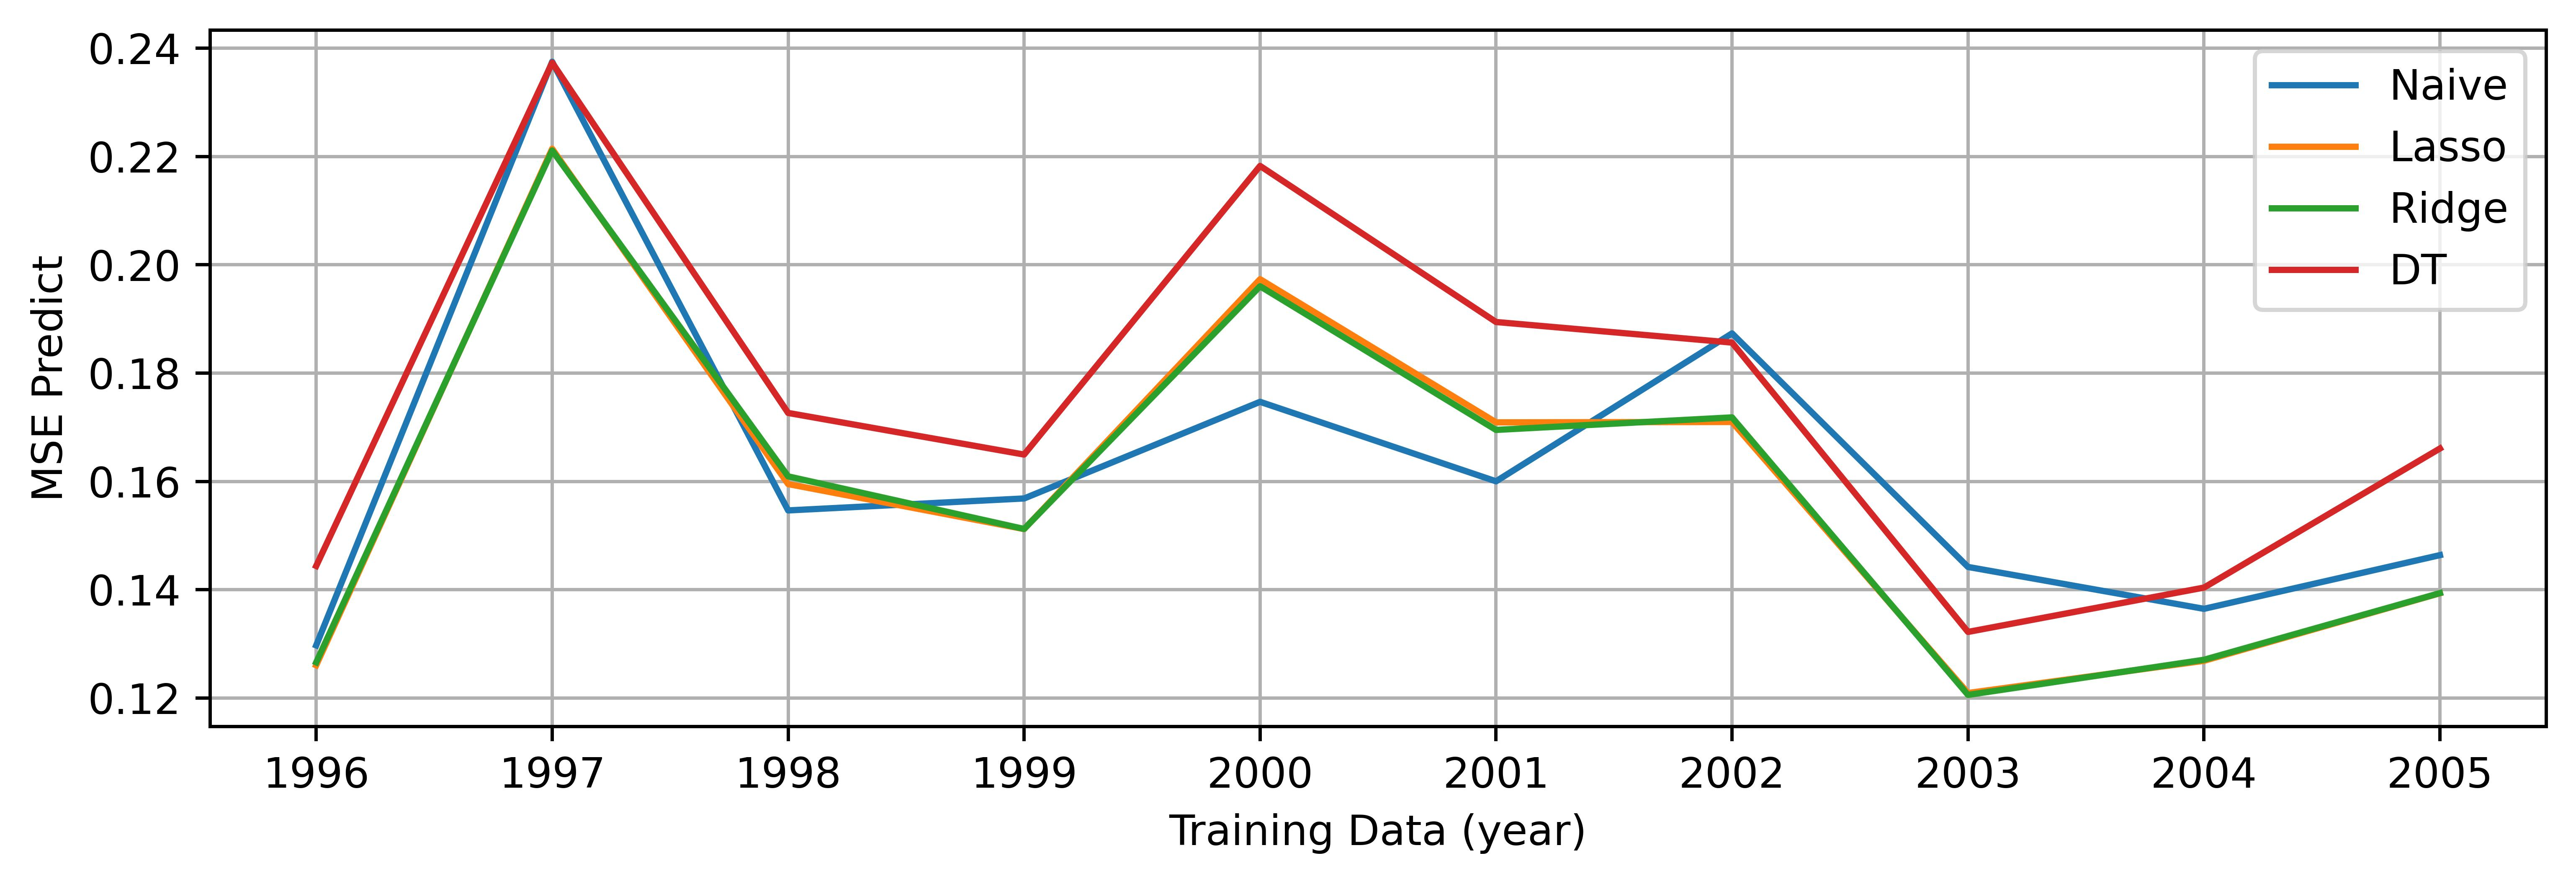
\includegraphics[width=0.7\textwidth]{../Result/Res-1_MSE_pred.jpg}
    \caption{MAE and MSE for predicting the following 1-year's data with the model trained by the previous 1-year's data.}
    \label{figure-1-year-pred}
  \end{figure}
  \clearpage
}

From the result, we can easily infer that the Lasso regression and Ridge regression can get almost the same error while the error of the decision tree is much higher. And all the models perform better when predicting the data of the same year rather than the following year. Furthermore, the prediction of the following year, especially the result of Lasso and Ridge regression, achieves much more accurate after 2002 with the enforcement of Sarbanes-Oxley Act, which implies that the this act might make the report more informative. Another noticeable different is that the error of predicting the following year gets worse in 2000, which may cause by the dot-com bubblt.

\subsubsection{Model trained by 1-year training data}

It is widely known that more training data can lead to a better method performance, with the assumption that all the data are from the same distribution. In this case, we presume that the information or the distribution of the words are similar across the nearby years. This assumption is reasonable, otherwise we can't expect the model to do the prediction. But it still needs to be certified.

Therefore we train the model with the data from nearby 3 year, and test the model on the same 3 year's data as well as the next year's data. The Figure \ref{figure-3-year-test} shows the error of the model predicting the volatility in the same 3 years, while the Figure \ref{figure-3-year-pred} shows the error of the prediction with the text and volatility of the following year.

\afterpage{
  \clearpage
  \begin{figure}[H]
    \centering
    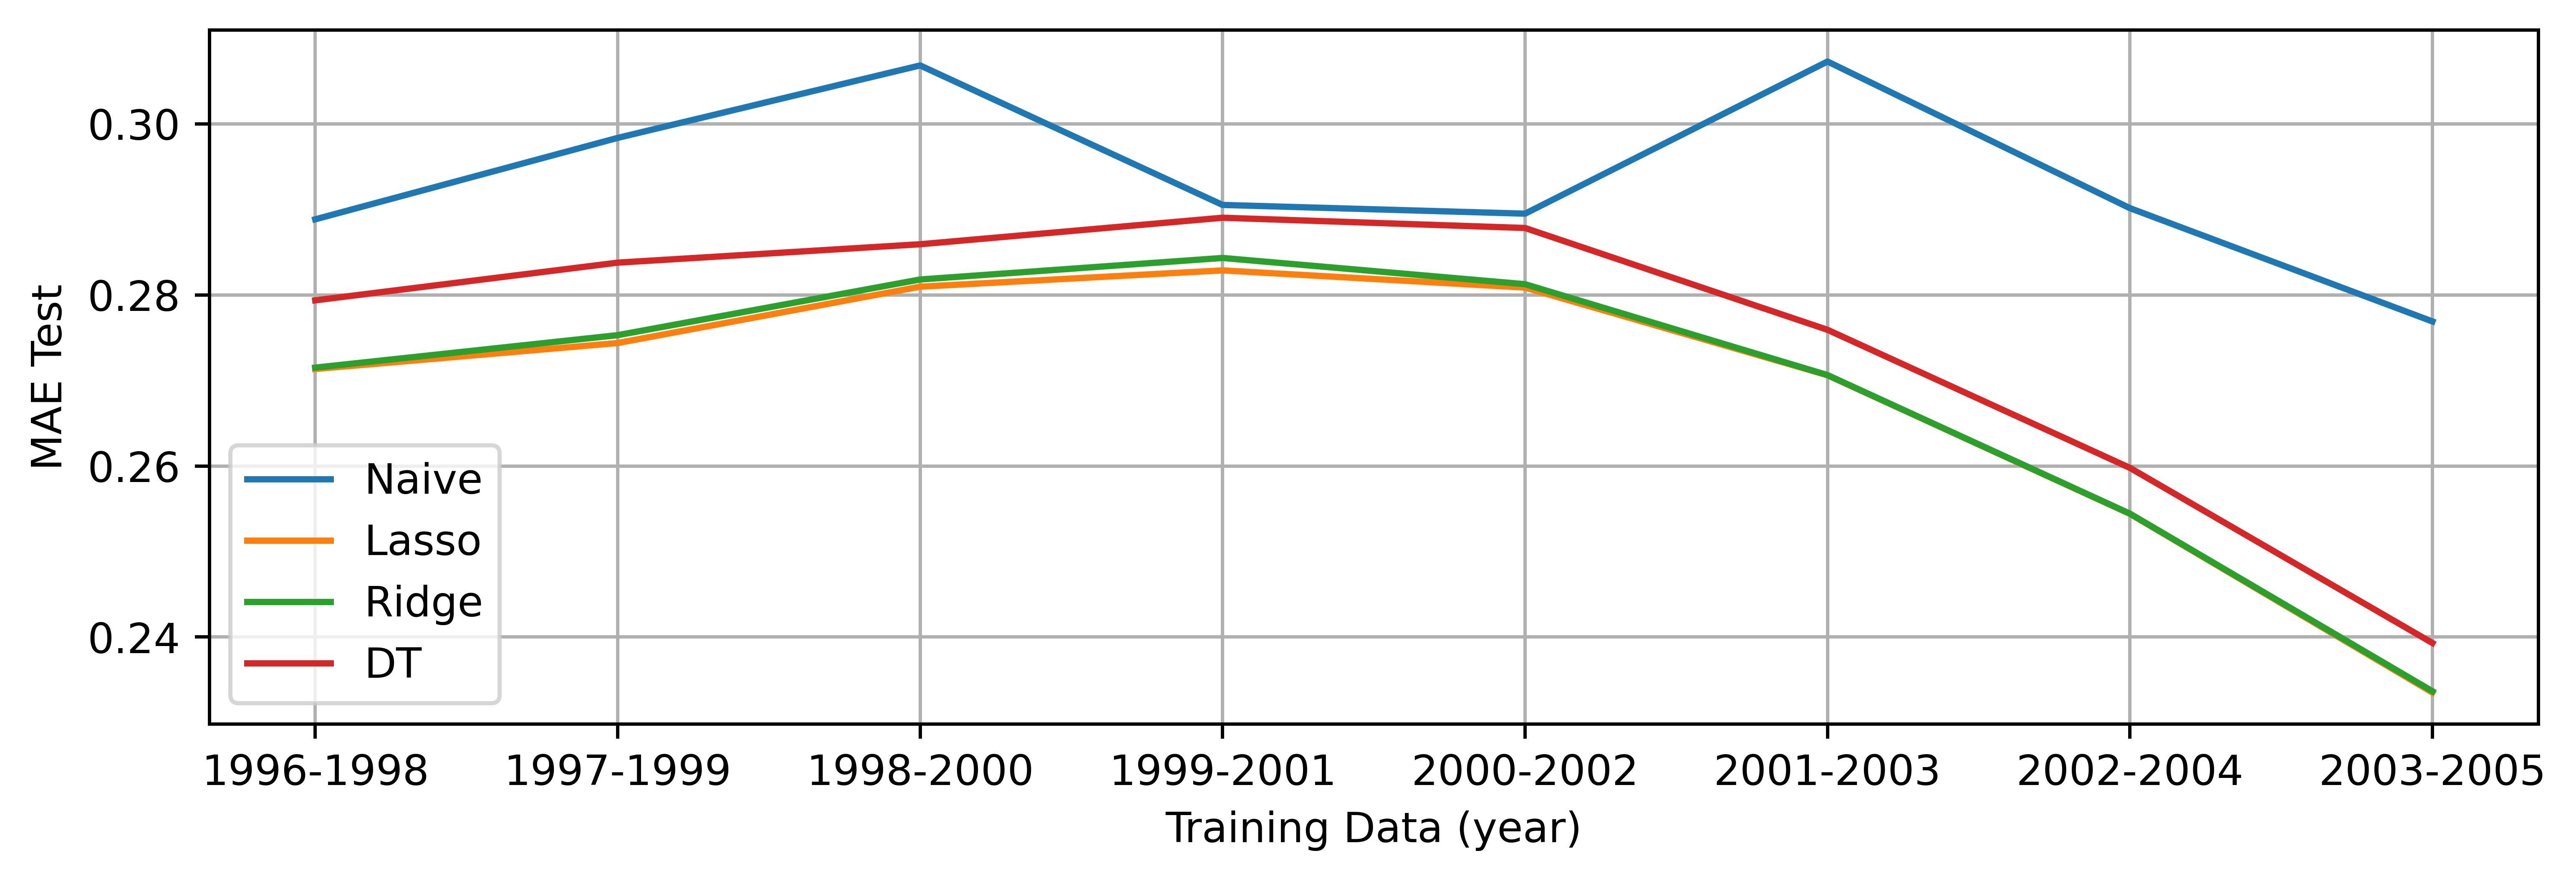
\includegraphics[width=0.7\textwidth]{../Result/Res-3_MAE_test.jpg} \\
    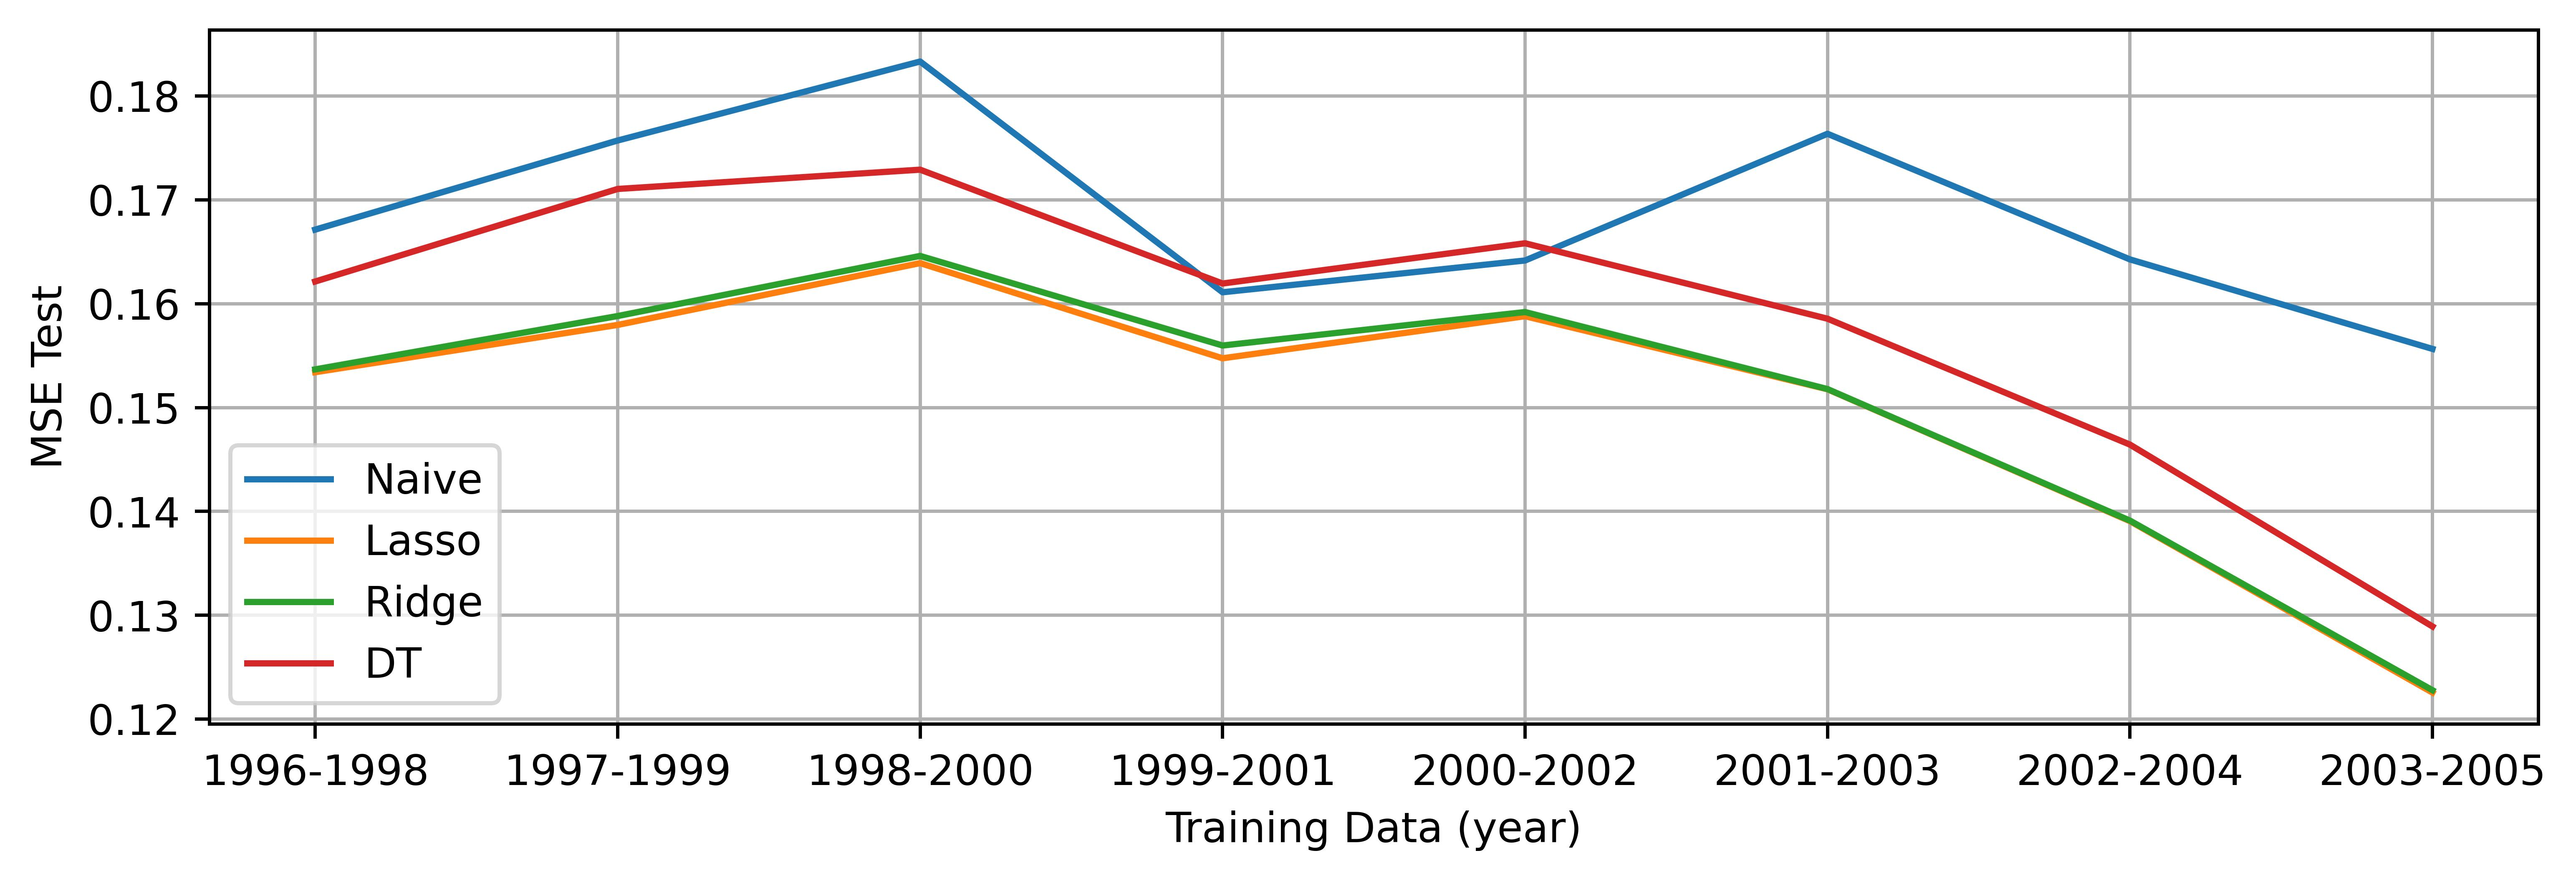
\includegraphics[width=0.7\textwidth]{../Result/Res-3_MSE_test.jpg}
    \caption{MAE and MSE for predicting the 3-year's data with the model trained by the same 3-year's data.}
    \label{figure-3-year-test}
  \end{figure}

  \begin{figure}[H]
    \centering
    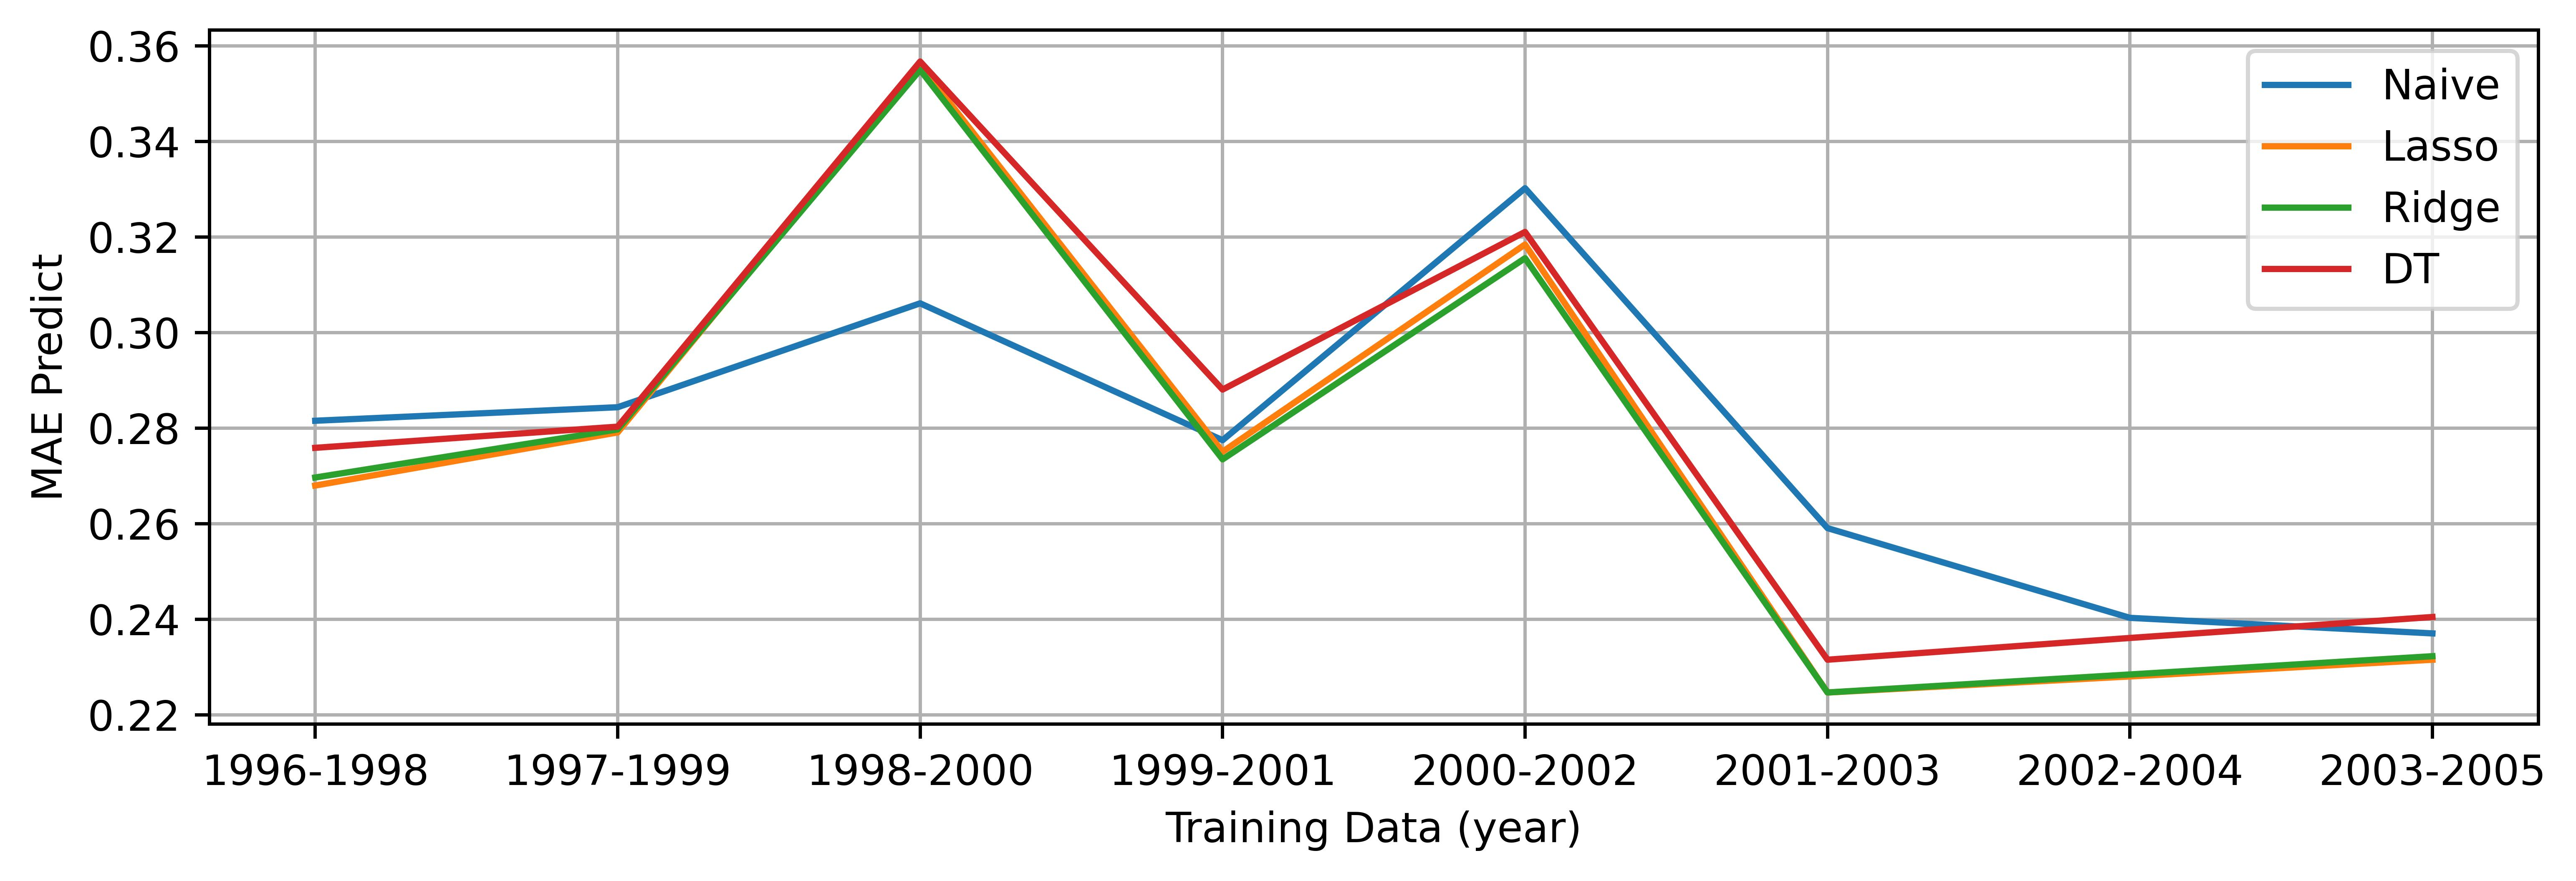
\includegraphics[width=0.7\textwidth]{../Result/Res-3_MAE_pred.jpg} \\
    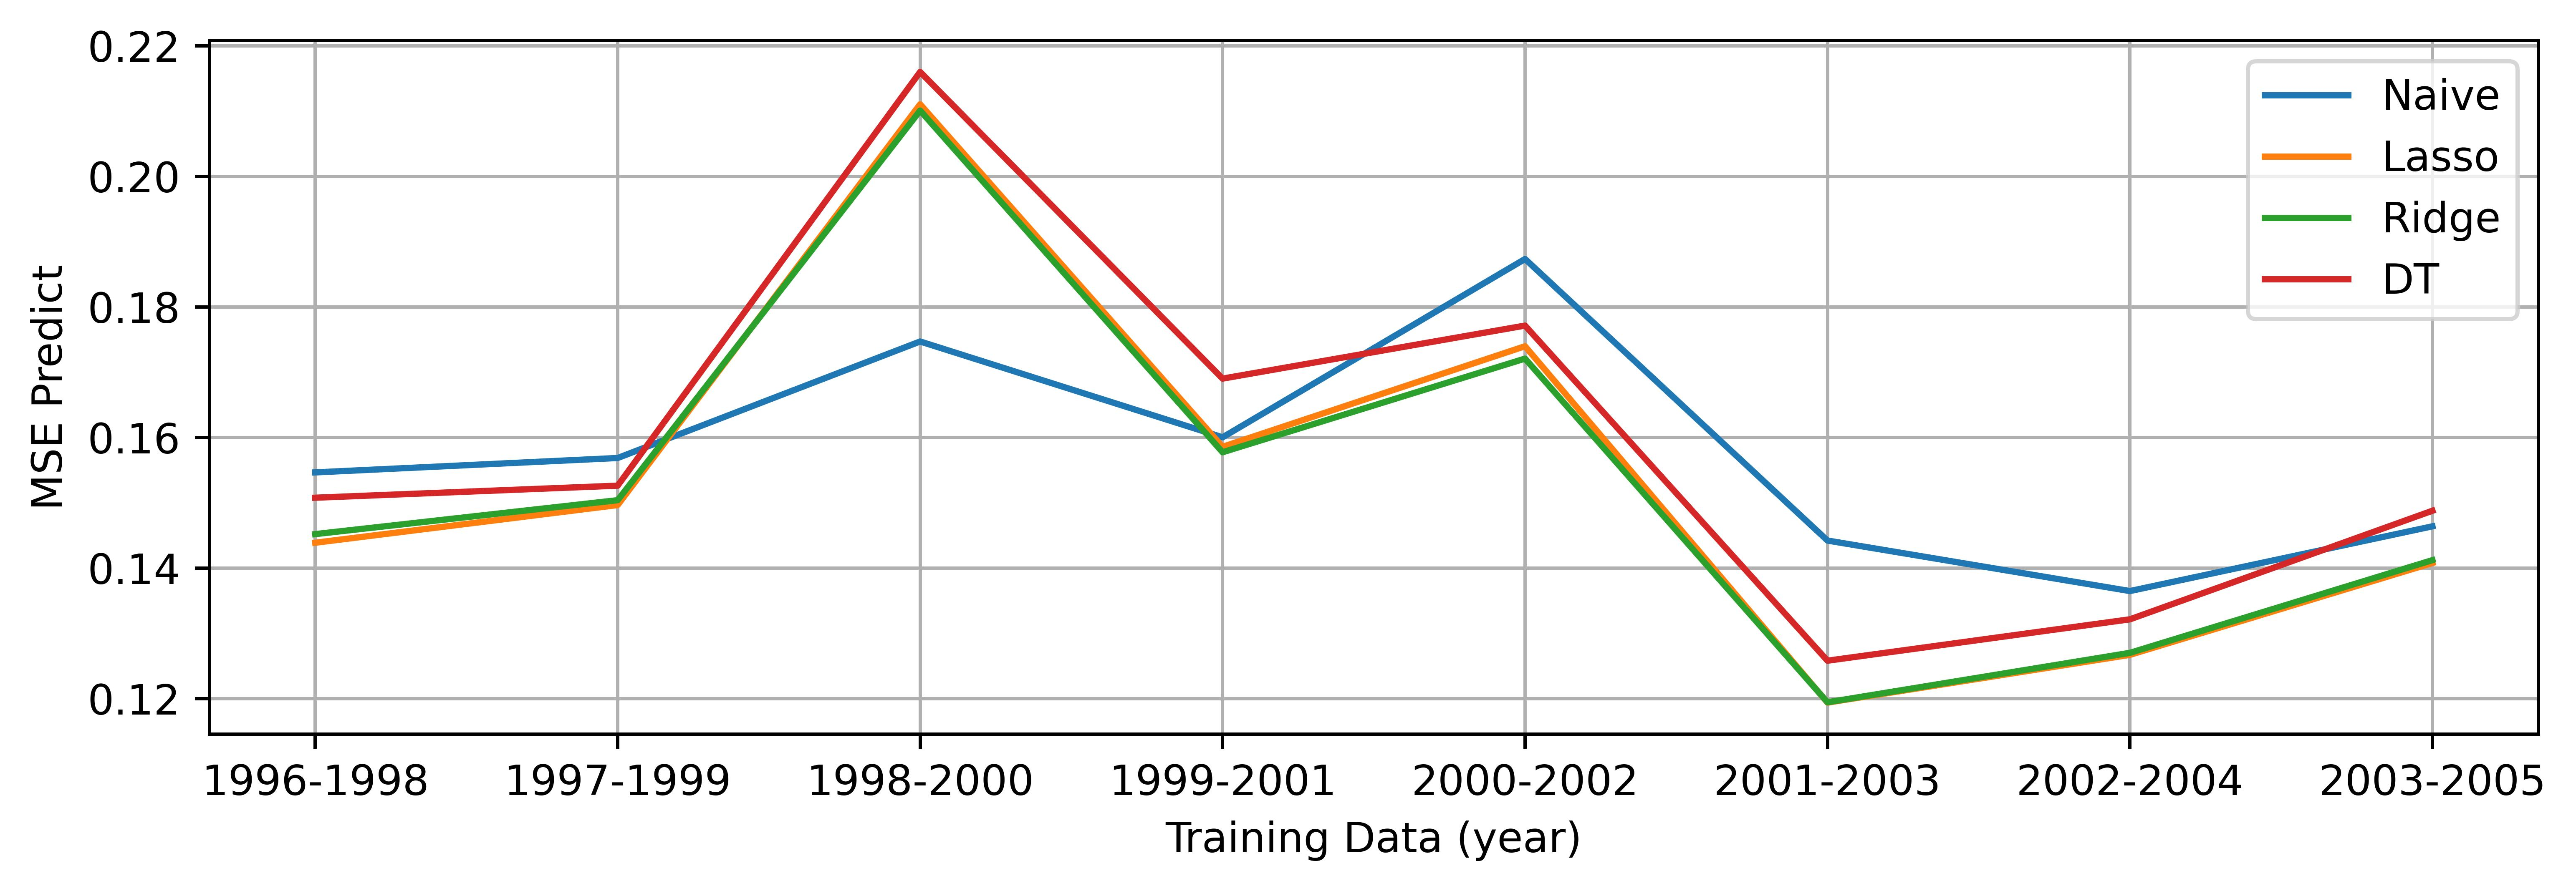
\includegraphics[width=0.7\textwidth]{../Result/Res-3_MSE_pred.jpg}
    \caption{MAE and MSE for predicting the following 1-year's data with the model trained by the previous 3-year's data.}
    \label{figure-3-year-pred}
  \end{figure}
  \clearpage
}

Similar to the 1-year training data, the result still shows the influence of the dot-com bubble and the Sarbanes-Oxley Act. Meanwhile, the errors of three models become more closer and more prediction are better than or equivalent to the Naive model, which implies the higher stability and higher accuracy than the model based on the 1-year's data.

\subsection{Wrod Features}

\afterpage{
  \clearpage
  \begin{table}[p]
    \centering
    \begin{tabular}{|c|c|c|c|c|}
      \hline
      Year                       & Method        & Increasing Common          & Decreasing Common          & Different                   \\
      \hline
      \multirow{3}{*}{1996-1997} & Lasso         & $53.9\%$                   & $60.6\%$                   & $1.9\%$                     \\
      \cline{2-5}
                                 & Ridge         & $48.3\%$                   & $55.1\%$                   & $2.9\%$                     \\
      \cline{2-5}
                                 & Decision Tree & $62.7\%$                   & $15.8\%$                   & $3.6\%$                     \\
      \hline
      \multirow{3}{*}{1997-1998} & Lasso         & $35.1\%$                   & $39.2\%$                   & $6.4\%$                     \\
      \cline{2-5}
                                 & Ridge         & $38.1\%$                   & $36.9\%$                   & $7.55\%$                    \\
      \cline{2-5}
                                 & Decision Tree & $46.2\%$                   & $29.4\%$                   & $6.75\%$                    \\
      \hline
      \multirow{3}{*}{1998-1999} & Lasso         & \textcolor{blue}{$23.6\%$} & $31.7\%$                   & $5.6\%$                     \\
      \cline{2-5}
                                 & Ridge         & \textcolor{blue}{$20.2\%$} & $32.1\%$                   & $8.35\%$                    \\
      \cline{2-5}
                                 & Decision Tree & $37.1\%$                   & $18.8\%$                   & $8.4\%$                     \\
      \hline
      \multirow{3}{*}{1999-2000} & Lasso         & \textcolor{red}{$3.8\%$}   & \textcolor{blue}{$27.8\%$} & \textcolor{blue}{$17.1\%$}  \\
      \cline{2-5}
                                 & Ridge         & \textcolor{red}{$9.9\%$}   & $38.6\%$                   & $6.55\%$                    \\
      \cline{2-5}
                                 & Decision Tree & $29.3\%$                   & $33.2\%$                   & $4.4\%$                     \\
      \hline
      \multirow{3}{*}{2000-2001} & Lasso         & \textcolor{red}{$5.1\%$}   & \textcolor{blue}{$24.9\%$} & $1.2\%$                     \\
      \cline{2-5}
                                 & Ridge         & \textcolor{red}{$13.2\%$}  & \textcolor{blue}{$18.9\%$} & $3.25\%$                    \\
      \cline{2-5}
                                 & Decision Tree & $23.9\%$                   & $32.7\%$                   & $6.2\%$                     \\
      \hline
      \multirow{3}{*}{2001-2002} & Lasso         & $38.0\%$                   & $30.4\%$                   & $2.7\%$                     \\
      \cline{2-5}
                                 & Ridge         & $42.2\%$                   & $35.7\%$                   & $4.15\%$                    \\
      \cline{2-5}
                                 & Decision Tree & $23.7\%$                   & \textcolor{red}{$3.6\%$}   & \textcolor{blue}{$10.9\%$}  \\
      \hline
      \multirow{3}{*}{2002-2003} & Lasso         & $31.7\%$                   & $31.0\%$                   & \textcolor{blue}{$12.15\%$} \\
      \cline{2-5}
                                 & Ridge         & $35.8\%$                   & $36.4\%$                   & $9.2\%$                     \\
      \cline{2-5}
                                 & Decision Tree & $45.7\%$                   & \textcolor{red}{$5.8\%$}   & $4.3\%$                     \\
      \hline
      \multirow{3}{*}{2003-2004} & Lasso         & \textcolor{blue}{$26.2\%$} & \textcolor{blue}{$58.3\%$} & $3.15\%$                    \\
      \cline{2-5}
                                 & Ridge         & \textcolor{blue}{$27.3\%$} & \textcolor{blue}{$44.6\%$} & $1.25\%$                    \\
      \cline{2-5}
                                 & Decision Tree & \textcolor{blue}{$34.7\%$} & \textcolor{red}{$2.0\%$}   & \textcolor{blue}{$11.85\%$} \\
      \hline
      \multirow{3}{*}{2004-2005} & Lasso         & $42.2\%$                   & $38.3\%$                   & $6.4\%$                     \\
      \cline{2-5}
                                 & Ridge         & $45.5\%$                   & $43.6\%$                   & $9.3\%$                     \\
      \cline{2-5}
                                 & Decision Tree & $56.7\%$                   & \textcolor{red}{$7.3\%$}   & $2.1\%$                     \\
      \hline
    \end{tabular}
    \caption{The rate of common and different word features across different years. The column ``Increasing Common" and ``Decreasing Common" shows the rate of the common features related to the increasing or decreasing volatility from nearby two years, the column ``Different" shows the rate of the features that are corresponding to the different trend in the two years, i.e. the rate of the features that changes the meanings. Values in red are outliers from the whole, and blue means the large gap from the previous and following year.}
    \label{table-words-feature-year}
  \end{table}
  \clearpage
}

Another problem we concern about is the words feature, especially whether they are different cross years or models. Thus we compare the words features given by different models with training data from different years. The Table \ref{table-words-feature-year} compares the words features across years, where the column ``Increasing Common" and ``Decreasing Common" shows the rate of the common features related to the increasing or decreasing volatility from nearby two years, the column ``Different" shows the rate of the features that are corresponding to the different trend in the two years, i.e. the rate of the features that changes the meanings.

This table shows that in the most of cases, the word features are similar between the nearby years, while there are some abnormal values, mostly around 2000 and 2003. The the abnormal values are corresponding to the year of the dot-com bubble and the Sarbanes-Oxley Act, which confirm the conclusion that the big events will affect the information or the distribution of the wrods, and it also shows that the firm are more likely to follow the act from 2003.

\afterpage{
  \clearpage
  \begin{table}[p]
    \centering
    \begin{tabular}{|c|c|c|c|c|}
      \hline
      Year                  & Compared Methods       & Increasing Common & Decreasing Common & Different \\
      \hline
      \multirow{3}{*}{1996} & Lasso \& Ridge         & $75.2\%$          & $71.6\%$          & $0.15\%$  \\
      \cline{2-5}
                            & Lasso \& Decision Tree & $23.2\%$          & $7.7\%$           & $27.0\%$  \\
      \cline{2-5}
                            & Ridge \& Decision Tree & $36.1\%$          & $25.1\%$          & $17.35\%$ \\
      \hline
      \multirow{3}{*}{1997} & Lasso \& Ridge         & $82.0\%$          & $87.2\%$          & $0.15\%$  \\
      \cline{2-5}
                            & Lasso \& Decision Tree & $15.4\%$          & $7.3\%$           & $25.85\%$ \\
      \cline{2-5}
                            & Ridge \& Decision Tree & $16.6\%$          & $12.2\%$          & $25.6\%$  \\
      \hline
      \multirow{3}{*}{1998} & Lasso \& Ridge         & $84.4\%$          & $85.5\%$          & $0.2\%$   \\
      \cline{2-5}
                            & Lasso \& Decision Tree & $14.1\%$          & $15.1\%$          & $15.4\%$  \\
      \cline{2-5}
                            & Ridge \& Decision Tree & $12.2\%$          & $15.6\%$          & $18.6\%$  \\
      \hline
      \multirow{3}{*}{1999} & Lasso \& Ridge         & $67.9\%$          & $83.9\%$          & $0.35\%$  \\
      \cline{2-5}
                            & Lasso \& Decision Tree & $17.8\%$          & $23.8\%$          & $19.8\%$  \\
      \cline{2-5}
                            & Ridge \& Decision Tree & $11.5\%$          & $23.1\%$          & $24.0\%$  \\
      \hline
      \multirow{3}{*}{2000} & Lasso \& Ridge         & $68.1\%$          & $55.3\%$          & $1.85\%$  \\
      \cline{2-5}
                            & Lasso \& Decision Tree & $19.0\%$          & $25.1\%$          & $17.6\%$  \\
      \cline{2-5}
                            & Ridge \& Decision Tree & $24.1\%$          & $9.5\%$           & $26.1\%$  \\
      \hline
      \multirow{3}{*}{2001} & Lasso \& Ridge         & $91.7\%$          & $92.9\%$          & $0.1\%$   \\
      \cline{2-5}
                            & Lasso \& Decision Tree & $5.5\%$           & $0.9\%$           & $31.55\%$ \\
      \cline{2-5}
                            & Ridge \& Decision Tree & $6.8\%$           & $1.6\%$           & $30.55\%$ \\
      \hline
      \multirow{3}{*}{2002} & Lasso \& Ridge         & $88.6\%$          & $79.1\%$          & $0.1\%$   \\
      \cline{2-5}
                            & Lasso \& Decision Tree & $37.7\%$          & $49.8\%$          & $9.75\%$  \\
      \cline{2-5}
                            & Ridge \& Decision Tree & $33.8\%$          & $39.2\%$          & $14.35\%$ \\
      \hline
      \multirow{3}{*}{2003} & Lasso \& Ridge         & $93.6\%$          & $89.5\%$          & $0.15\%$  \\
      \cline{2-5}
                            & Lasso \& Decision Tree & $13.4\%$          & $10.4\%$          & $27.05\%$ \\
      \cline{2-5}
                            & Ridge \& Decision Tree & $15.2\%$          & $13.9\%$          & $25.45\%$ \\
      \hline
      \multirow{3}{*}{2004} & Lasso \& Ridge         & $75.2\%$          & $73.4\%$          & $0.2\%$   \\
      \cline{2-5}
                            & Lasso \& Decision Tree & $23.5\%$          & $24.2\%$          & $21.25\%$ \\
      \cline{2-5}
                            & Ridge \& Decision Tree & $30.4\%$          & $20.4\%$          & $20.85\%$ \\
      \hline
      \multirow{3}{*}{2005} & Lasso \& Ridge         & $95.6\%$          & $90.8\%$          & $0.4\%$   \\
      \cline{2-5}
                            & Lasso \& Decision Tree & $9.9\%$           & $2.5\%$           & $27.5\%$  \\
      \cline{2-5}
                            & Ridge \& Decision Tree & $10.2\%$          & $5.2\%$           & $28.7\%$  \\
      \hline
    \end{tabular}
    \caption{The rate of common and different word features across different models. The column ``Increasing Common" and ``Decreasing Common" shows the rate of the common features related to the increasing or decreasing volatility from nearby two years, the column ``Different" shows the rate of the features that are corresponding to the different trend in the two years, i.e. the rate of the features that changes the meanings.}
    \label{table-words-feature-model}
  \end{table}
}

The Table \ref{table-words-feature-model} compares the word features given by different models. Similar to the previous, we compute the rate of the common features and different features. It is easy to see that the Lasso and Ridge regression shares most of the features, while the decision tree gives the totally different features.

We try to figure out the reason behind this phenomena by analyse the coefficients  given by the models. The parameter shows that the decisionn tree puts a higher importance on the historical volatility, while the Lasso and Ridge regression gives a much more averagely coefficients. For example, with the training data from 1996, the decision tree will give all the importance of word features less than $0.1$, while those given by the Lasso and Ridge regression can be up to $0.5$. This might be caused by many reasons, but we believe that the most important one is that the decision tree is in fact non linear, thus when it tries to fit the data, it will obviously concern more on the historical volatility as it will be much more significantly different compare with the word features. One possible way to reduce this is to predict the difference of the volatility, or simply do the classification on the trend, which can be used in further research.

\section{Conclusion}

We applied the Lasso regression, Ridge regression, and decision tree to the companies' 10-K report, as well as the historical volatility, to forecast the volatility. Similar to the previous research\cite{kogan2009predicting}, our result also shows that the 10-K report, especially the report after the Sarbanes–Oxley Act, can help to predict the value better than the naive model, and more training data can lead to a better model performance. Furthermore, big events like the dot-com bubble and the Sarbanes-Oxley Act can make a significant effect on the information or the distribution of the text.

\newpage

\bibliographystyle{unsrt}
\bibliography{reference.bib}
\addcontentsline{toc}{section}{References}

\newpage

\appendix
\renewcommand\thesection{\Alph{section}}

\section{Author Contributions}



\end{document}